\documentclass[color=usenames,dvipsnames]{beamer}\usepackage[]{graphicx}\usepackage[]{color}
% maxwidth is the original width if it is less than linewidth
% otherwise use linewidth (to make sure the graphics do not exceed the margin)
\makeatletter
\def\maxwidth{ %
  \ifdim\Gin@nat@width>\linewidth
    \linewidth
  \else
    \Gin@nat@width
  \fi
}
\makeatother

\definecolor{fgcolor}{rgb}{0.345, 0.345, 0.345}
\newcommand{\hlnum}[1]{\textcolor[rgb]{0.686,0.059,0.569}{#1}}%
\newcommand{\hlstr}[1]{\textcolor[rgb]{0.192,0.494,0.8}{#1}}%
\newcommand{\hlcom}[1]{\textcolor[rgb]{0.678,0.584,0.686}{\textit{#1}}}%
\newcommand{\hlopt}[1]{\textcolor[rgb]{0,0,0}{#1}}%
\newcommand{\hlstd}[1]{\textcolor[rgb]{0.345,0.345,0.345}{#1}}%
\newcommand{\hlkwa}[1]{\textcolor[rgb]{0.161,0.373,0.58}{\textbf{#1}}}%
\newcommand{\hlkwb}[1]{\textcolor[rgb]{0.69,0.353,0.396}{#1}}%
\newcommand{\hlkwc}[1]{\textcolor[rgb]{0.333,0.667,0.333}{#1}}%
\newcommand{\hlkwd}[1]{\textcolor[rgb]{0.737,0.353,0.396}{\textbf{#1}}}%
\let\hlipl\hlkwb

\usepackage{framed}
\makeatletter
\newenvironment{kframe}{%
 \def\at@end@of@kframe{}%
 \ifinner\ifhmode%
  \def\at@end@of@kframe{\end{minipage}}%
  \begin{minipage}{\columnwidth}%
 \fi\fi%
 \def\FrameCommand##1{\hskip\@totalleftmargin \hskip-\fboxsep
 \colorbox{shadecolor}{##1}\hskip-\fboxsep
     % There is no \\@totalrightmargin, so:
     \hskip-\linewidth \hskip-\@totalleftmargin \hskip\columnwidth}%
 \MakeFramed {\advance\hsize-\width
   \@totalleftmargin\z@ \linewidth\hsize
   \@setminipage}}%
 {\par\unskip\endMakeFramed%
 \at@end@of@kframe}
\makeatother

\definecolor{shadecolor}{rgb}{.97, .97, .97}
\definecolor{messagecolor}{rgb}{0, 0, 0}
\definecolor{warningcolor}{rgb}{1, 0, 1}
\definecolor{errorcolor}{rgb}{1, 0, 0}
\newenvironment{knitrout}{}{} % an empty environment to be redefined in TeX

\usepackage{alltt}
%\documentclass[color=usenames,dvipsnames,handout]{beamer}

%\usepackage[roman]{../pres1}
\usepackage[sans]{../pres1}
\usepackage{graphicx}
\usepackage{bm}
%\usepackage{changepage}
\usepackage{tikz}
\usetikzlibrary{shapes,arrows,snakes,backgrounds}




\IfFileExists{upquote.sty}{\usepackage{upquote}}{}
\begin{document}


\setlength{\fboxsep}{0pt}


\begin{frame}[plain]
  \begin{center}
    {\LARGE \bf Age- and stage-structured population models \\}
    \vfill
%    \fbox{
      \fbox{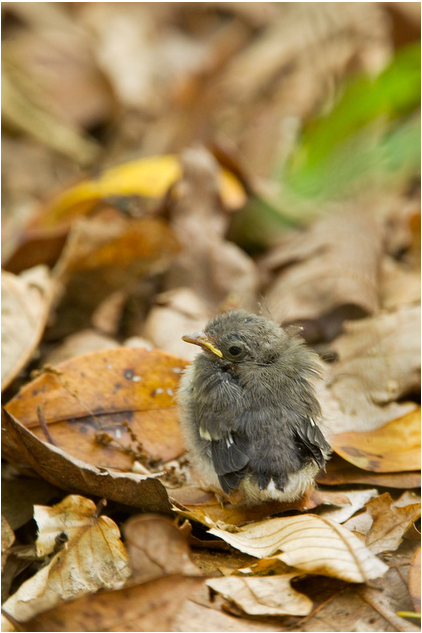
\includegraphics[height=2.7cm,keepaspectratio]{figs/AMRE-HY-male}} \hfill
      \fbox{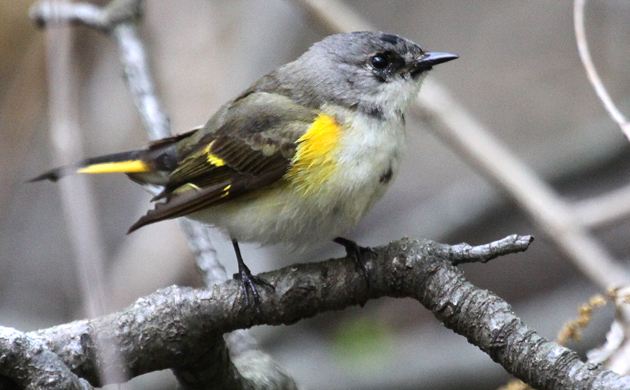
\includegraphics[height=2.7cm,keepaspectratio]{figs/AMRE-SY-male}} \hfill
      \fbox{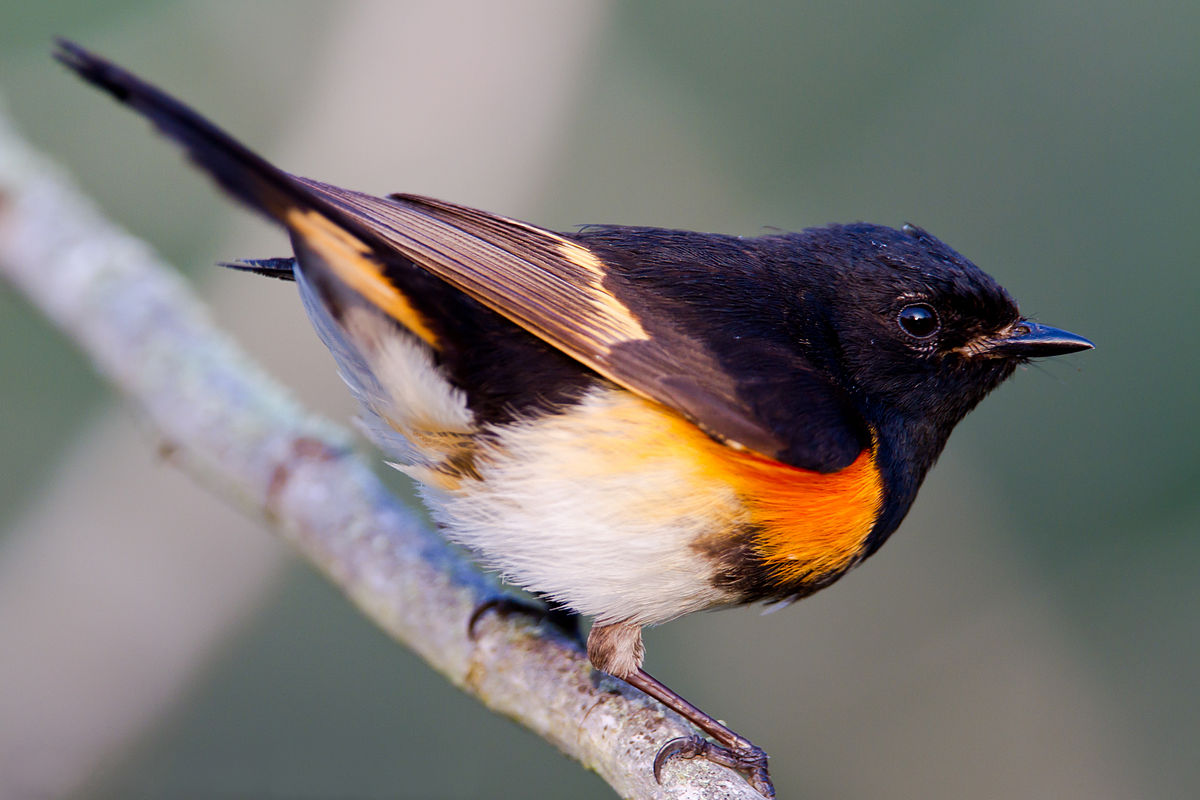
\includegraphics[height=2.7cm,keepaspectratio]{figs/AMRE-ASY-M}}
%    }
  \end{center}
\end{frame}





\section{Introduction}


\begin{frame}[plain]
  \frametitle{Today's topics}
%  {\huge Today's topics}
  \tableofcontents%[currentsection]
\end{frame}



\begin{frame}
  \frametitle{Motivation}
  \large
%  \begin{itemize}[<+->]
%  \item
  Birth and death rates usually depend on age. \\
  \pause
  \vfill
  % \item
  Growth rates will differ between populations with
  different age structures. \\
  \pause
  \vfill
  % \item
  Some age classes contribute more to population growth than others. \\
  \pause
  \vfill
  % \item
  These facts have important management implications. \\
%    \item Harvesting larger numbers of the age group that most
%      positively influences population growth = bad idea
%    \item If habitat degradation affects an influential age group, we may be putting the
%      population at risk
%    \item  Will be more successful if we re-establish the most influential age group
%    \item Population control - May want to target the most influential age group for
%      elimination
%    \item Take Home - Determining the most influential age is of paramount importance for
%      knowing what management actions should be conducted!
%  \end{itemize}
\end{frame}



\begin{frame}
  \frametitle{Matrix models vs life tables}
  \begin{columns}
%    \large
    \begin{column}[T]{0.5\textwidth}
      {\bf Matrix models}
      \begin{itemize}
        \item<1-> Age is discrete
        \item<2-> Age class is denoted by $i$
%        \item<3-> Individuals either advance to the next age class or die
%        \item<3-> An age class is not necessarily a 1 year time period
        \item<3-> Each age class can have its own vital rates
%        \item We usually only care about females
      \end{itemize}
    \end{column}
    \begin{column}[T]{0.5\textwidth}
      {\bf Life tables}
      \begin{itemize}
        \item<1-> Age is continuous
        \item<2-> Actual age is denoted by $x$
        \item<3-> Each age can have its own vital rates
      \end{itemize}
    \end{column}
  \end{columns}
  \begin{center}
    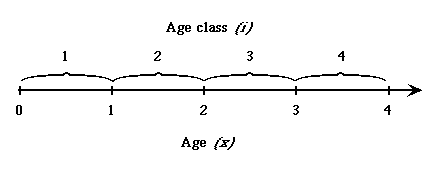
\includegraphics[width=0.9\textwidth]{figs/age-class-diagram}
  \end{center}
\end{frame}



%% \begin{frame}[fragile]
%%   \frametitle{Scenario}
%% <<age-diagram,echo=FALSE,fig=FALSE>>=
%% plot(0,0, pch=NA, frame=FALSE, axes=FALSE, ann=FALSE, xlim=c(0, 5), ylim=c(-1, 1))
%% arrows(0, 0, 5, 0)
%% text(0.5, 0.2, "}", cex=5, srt=90, family = 'Helvetica Neue UltraLight')
%% @
%% \end{frame}



%\note{simple example with adult and juvenile age classes}
%\note{birth flow vs birth pulse}
%\note{postbreeding vs prebreeding census}
%\note{In these models, the transition of age cohorts through time is a
%  function of fixed survival and reproduction parameters}



%% \begin{frame}
%%   \frametitle{Conceptual model}
%%   \begin{center}
%%     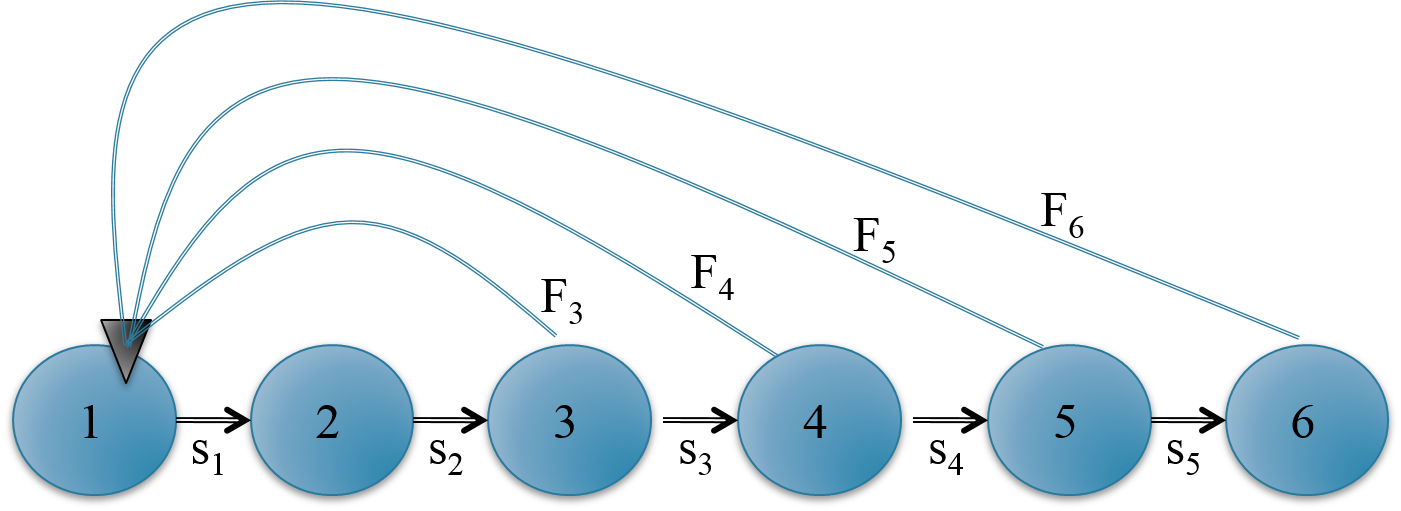
\includegraphics[width=0.9\textwidth]{figs/age-diagram1}
%%   \end{center}
%% \end{frame}





\begin{frame}
  \frametitle{Age-class abundance and age distribution}
  \large
  \begin{itemize}%[<+->]
    \item $n_{i,t}$ is abundance of age class $i$ in year $t$
    \item[]
    \item<2-> Suppose initial abundance in the 3 age classes is:
      \begin{itemize} \large
        \item $n_{1,0} = 50$ (Age class 1, juveniles)
        \item $n_{2,0} = 40$ (Age class 2, subadults)
        \item $n_{3,0} = 10$ (Age class 3, adults)
      \end{itemize}
    \item[]
    \item<3-> This implies an initial age distribution of:
      \begin{itemize} \large
%        \item  $c_{1,0} = n_{1,0}/\sum_{i=1}^3 n_{i,0} = 0.5$
%        \item  $c_{2,0} = n_{2,0}/\sum_{i=1}^3 n_{i,0} = 0.4$
%        \item  $c_{3,0} = n_{3,0}/\sum_{i=1}^3 n_{i,0} = 0.1$
        \item  $c_{1,0} = n_{1,0}/N_0 = 0.5$
        \item  $c_{2,0} = n_{2,0}/N_0 = 0.4$
        \item  $c_{3,0} = n_{3,0}/N_0 = 0.1$
      \end{itemize}
  \end{itemize}
  \vfill
  \uncover<4->{
  {\centering \bf An age distribution describes the proportion of
    individuals in each age class \\}
  }
\end{frame}




\begin{frame}[fragile]
  \frametitle{Age distribution}
%  \begin{center}
\begin{knitrout}
\definecolor{shadecolor}{rgb}{0.969, 0.969, 0.969}\color{fgcolor}

{\centering \includegraphics[width=0.85\textwidth]{figure/struc1-1} 

}



\end{knitrout}
%  \end{center}
\end{frame}




\begin{frame}
  \frametitle{Age distribution}
  {\centering \bf Declining populations have relatively more old individuals than
  growing populations \\}
  \begin{center}
    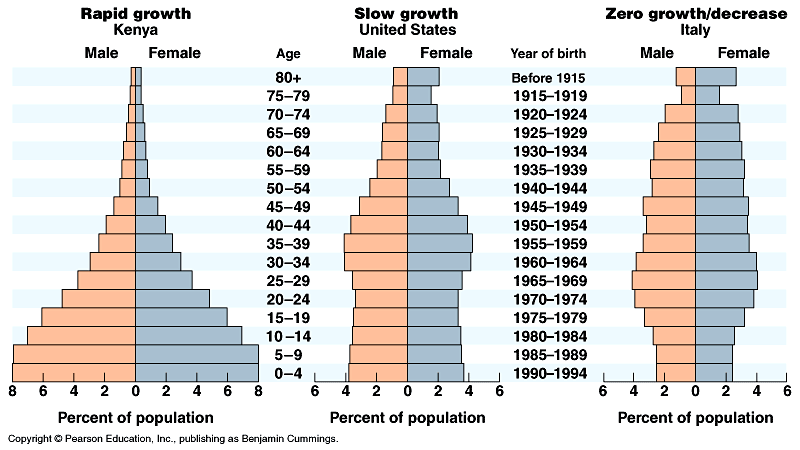
\includegraphics[width=\textwidth]{figs/AgeStructures}
  \end{center}
\end{frame}





\begin{frame}
  \frametitle{Three age class example}
%  {\bf How does this population grow? \par}
%  \vspace{5mm}
%  \large
  {\bf We need a model for $n_{i,t+1}$, abundance of each age class in
    next time step}
  \begin{itemize}
    \item Depends on age class survival rates $s_{i}$
    \item And age class birth rates $b_{i}$
    \item<3> Fecundity is often defined as the product of birth rate and offspring survival, $f_i = b_i
      \times s_0$
%    \item Note the lack of $t$ subscripts (for now)
  \end{itemize}
  \vspace{0.5cm}
  \pause
  \tikzstyle{level 1} = [circle, draw, text width=1cm, minimum size=2cm,
  node distance=4cm, text centered, fill=blue!10]
  \begin{center}
    \only<2 | handout:0>{
    \begin{tikzpicture}
      \node [level 1] (n1) [yshift=-5mm] {$n_{1,t}$};
      \node [level 1, right of=n1] (n2) [yshift=0mm] {$n_{2,t}$};
      \node [level 1, right of=n2] (n3) [yshift=0mm] {$n_{3,t}$};
      \draw[->,thick]  (n1) to node[above] {$s_1$} (n2);
      \draw[->,thick] (n2) to node[above] {$s_2$} (n3);
      \draw[->,thick] (n2) to [bend right=40] node[above] {$b_2 \times s_0$} (n1);
      \draw[->,thick] (n3) to [bend right=60] node[above] {$b_3 \times s_0$} (n1);
   \end{tikzpicture}
   } %\\
   \uncover<3>{
   \begin{tikzpicture}
      \node [level 1] (n1) [yshift=-5mm] {$n_{1,t}$};
      \node [level 1, right of=n1] (n2) [yshift=0mm] {$n_{2,t}$};
      \node [level 1, right of=n2] (n3) [yshift=0mm] {$n_{3,t}$};
      \draw[->,thick]  (n1) to node[above] {$s_1$} (n2);
      \draw[->,thick] (n2) to node[above] {$s_2$} (n3);
      \draw[->,thick] (n2) to [bend right=40] node[above] {$f_2$} (n1);
      \draw[->,thick] (n3) to [bend right=60] node[above] {$f_3$} (n1);
   \end{tikzpicture}
   } %\\
  \end{center}
\end{frame}



\begin{frame}
  \frametitle{How does this population grow?}
  \large
  \begin{center}
    \begin{tabular}{cl}
      \hline
      Age class & Equation \\
      \hline
      1 & $n_{1,t+1} = n_{1,t} \times f_1 + n_{2,t} \times f_2 + n_{3,t} \times f_3$ \\ \pause
      2 & $n_{2,t+1} = n_{1,t} \times s_{1}$ \\ \pause
      3 & $n_{3,t+1} = n_{2,t} \times s_{2}$ \\
      \hline
    \end{tabular}
  \end{center}
  \normalsize
  \pause
  \vfill
  According to this model, all animals die after spending one time interval in the third age class. \\
  \pause
  \vfill
  In stage-structured models, animals can stay in an age class for more than one time interval.
\end{frame}





\begin{frame}
  \frametitle{Example}
  \begin{center} \large
    Let's choose values of $s_i$ and $f_i$
  \end{center}
  \small
  \begin{tabular}{cccc}
    \hline
    Age class & Initial population size & Survival probability & Fecundity rate \\
              & $n_{i,0}$  & $s_i$ & $f_i$ \\
    \hline
    1 & 50 & 0.5 & 0.0  \\
    2 & 40 & 0.6 & 0.8  \\
    3 & 10 & 0.0 & 1.7  \\
    \hline
  \end{tabular}
\end{frame}






%% \begin{frame}
%%   \frametitle{Fecundity ($f_i$)}
%%   \Large
%%   \[
%%     f_i = s_i \times b_i
%%   \]
%%   \begin{itemize}[<+->]
%%     \item Fecundity ($f_i$) is the expected number of offspring
%%       produced by age class $i$
%%     \item Function of both survival and birth rates%Not quite the same thing as the birth rate ($b$)
%% %     \item We work with fertilities because individuals breed at the end of
%% %      the age class interval, so
%%   \end{itemize}
%% \end{frame}







\begin{frame}[fragile]
  \frametitle{Population size, $n_{i,t}$}

\vspace{-0.9cm}
\begin{center}
  \includegraphics[width=0.85\textwidth]{figure/proj1-1}
\end{center}
\end{frame}




\begin{frame}[fragile]
  \frametitle{Growth rates, $n_{i,t+1}/n_{i,t} = \lambda_{i,t}$}

\vspace{-0.9cm}
\begin{center}
  \includegraphics[width=0.85\textwidth]{figure/lambda1-1}
\end{center}
\end{frame}




\begin{frame}[fragile]
  \frametitle{Age distribution, $c_{i,t}$}

\vspace{-0.9cm}
\begin{center}
  \includegraphics[width=0.85\textwidth]{figure/prop1-1}
\end{center}
\end{frame}









\begin{frame}
  \frametitle{Important things to note}
  \large
%  \begin{itemize}[<+->]
%  \item
  Age distribution converges to a {\bf stable age
    distribution} when survival and fecundity rates are constant. \\
  \pause
  \vfill
  % \item
  Stable age distribution is the proportion of individuals in each age
  class when the population converges. \\
  \pause
  \vfill
  % \item
  Growth rates of each age class differ at first, but converge
  once the stable age distribution is reached. \\
  \pause
  \vfill
  % \item
  Asymptotic growth rate is $\lambda$ (without subscript). \\
  \pause
  \vfill
  % \item
  Growth rate at the stable age distribution is the same for
  all age classes, and it is geometric! \\
%    \item But abundance continues to change
%  \end{itemize}
\end{frame}







%\begin{frame}
%  \frametitle{Age class growth rates}
%
%\end{frame}




%% \begin{frame}
%%   \frametitle{Age Structure}
%%   \begin{itemize}[<+->]
%%     \item Age structure is characterized by an age distribution
%%     \item Age distribution is the proportion of individuals in each
%%       age class
%%   \end{itemize}
%% \end{frame}






%% \begin{frame}
%%   \frametitle{Stable age distribution}
%%   \large
%%   \begin{itemize}[<+->]
%% %    \item An age distribution is the proportion of individuals in each
%% %      age class
%%     \item When birth and death rates are constant, population will
%%       converge to stable age distribution, regardless of initial
%%       population size
%%     \item In the stable age distribution, the proportion of
%%       individuals in each age class remains constant
%%     \item In the stable age distribution, the absolute number of
%%       individuals is not constant unless $r=0$.
%%   \end{itemize}
%% \end{frame}



%% \begin{frame}[fragile]
%%   \frametitle{Age distribution of humans}
%% <<human-age>>=
%% w = c(0.1252, 0.1189, 0.1131, 0.1075)
%% @
%% \end{frame}


%\note{age distribution, stable age distribution}


%\note{We usually work with females}









\section{Matrix Models}



\begin{frame}
  \frametitle{Matrix models}
  \Large
%  \begin{itemize}[<+->]
%  \item
  Matrix models aren't actually ``new'' models. \\
  \pause
  \vfill
  % \item
  They are the same old models we have been talking about. \\
  \pause
  \vfill
  % \item
  But, they make it much easier to compute important
  quantities like $\lambda$ and {\it reproductive value}. \\
%    \item Everyone will think you are cool if you know what a Leslie
%      matrix is
%  \end{itemize}
\end{frame}



\begin{frame}
  \frametitle{What is a matrix?}
  {\bf Definition}: A matrix is a rectangular array of numbers
  \begin{itemize}
    \item Usually denoted by an uppercase, bold letter
    \item Either square or rounded brackets are used
    \item Usually, rows are indexed by $i$, columns by $j$
  \end{itemize}
  \pause

  \vspace{1cm}
  Example of a $3 \times 4$ matrix: \par
  \begin{center}
    \Large
    \[
    { \bf A} =
    \begin{bmatrix}
      a_{1,1} & a_{1,2} & a_{1,3} & a_{1,4} \\
      a_{2,1} & a_{2,2} & a_{2,3} & a_{2,4} \\
      a_{3,1} & a_{3,2} & a_{3,3} & a_{3,4}
    \end{bmatrix}
    \]
  \end{center}
\end{frame}


\begin{frame}
  \frametitle{Leslie matrix}
  \large
  {\bf What is it?}
  \begin{itemize}
    \item Square matrix %$s \times s$
    \item Fertilities on first row
    \item Survival probs on lower off-diagonal
  \end{itemize}
  \pause
  \vspace{.8cm}
  Example:
  \large
  \begin{center}
    \[
    {\bf A} =
    \begin{bmatrix}
      f_1 & f_2 & f_3 & f_4 \\
      s_1 & 0 & 0 & 0 \\
      0 & s_2 & 0 & 0 \\
      0 & 0 & s_3 & 0
    \end{bmatrix}
    \]
  \end{center}
\end{frame}






%\note{projection matrix}





\begin{frame}
  \frametitle{How do we use a Leslie matrix?}
  \large
  These two expressions are equivalent: \par
  \vspace{0.5cm}
  \begin{tabular}{cl}
    \hline
    Age class & Equation \\
    \hline
    1 & $n_{1,t+1} = n_{1,t} \times f_{1} + n_{2,t} \times f_{2} + n_{3,t} \times f_3$ \\
    2 & $n_{2,t+1} = n_{1,t} \times s_{1}$ \\
    3 & $n_{3,t+1} = n_{2,t} \times s_{2}$ \\
    \hline
  \end{tabular}
  \vfill
  {\centering AND \par}
  \vfill
  \[
    {\bf n}_{t+1} = {\bf A}\times {\bf n}_{t}
  \]
\end{frame}



\begin{frame}
  \frametitle{Matrix multiplication}
  \Large
  \begin{center}
    \[
    \uncover<2>{ %\pause
    \begin{bmatrix}
      aw + bx + cy + dz \\
      ew + fx + gy + hz \\
      iw + jx + ky + lz \\
      mw + nx + oy + pz
    \end{bmatrix}
    } =
    \begin{bmatrix}
      a & b & c & d \\
      e & f & g & h \\
      i & j & k & l \\
      m & n & o & p
    \end{bmatrix}
    \times
    \begin{bmatrix}
      w \\
      x \\
      y \\
      z
    \end{bmatrix}
    \]
  \end{center}
\end{frame}






\begin{frame}
  \frametitle{Matrix multiplication and Leslie matrix}
  \Large
  \begin{center}
    \[
    \begin{bmatrix}
      n_{1,t+1} \\
      n_{2,t+1} \\
      n_{3,t+1} \\
      n_{4,t+1}
    \end{bmatrix}
    =
    \begin{bmatrix}
      f_1 & f_2 & f_3 & f_4 \\
      s_1 & 0 & 0 & 0 \\
      0 & s_2 & 0 & 0 \\
      0 & 0 & s_3 & 0
    \end{bmatrix}
    \times
    \begin{bmatrix}
      n_{1,t} \\
      n_{2,t} \\
      n_{3,t} \\
      n_{4,t}
    \end{bmatrix}
    \]
  \end{center}
\end{frame}












% \begin{frame}
%   \frametitle{Other uses of the Leslie matrix}
%   \Large
%   \begin{itemize}[<+->]
%     \item The dominant eigenvalue is the growth rate $\lambda$
%     \item The right eigenvector is the {\bf stable age distribution}
%     \item The left eigenvector is {\bf Fisher's reproductive value}
%   \end{itemize}
% \end{frame}

















\section{Reproductive value}




%% \begin{frame}
%%   \frametitle{Net reproductive rate $R_0$}
%%   {\bf Definition}:  The average number of age class zero offspring
%%   produced by an average newborn organism during its lifetime
%%   \pause
%%   \[
%%     R_0 =
%%   \]
%% \end{frame}



\begin{frame}
  \frametitle{Reproductive Value}
  \large
%  {\bf Definition}: the number of future offspring expected
%  to be produced by an individual in age class $i$ over its remaining life
%  span, adjusted by the growth rate of the population \par
  {\bf Definition}: The extent to which an individual in age class
  $i$ will contribute to the ancestry of future generations. \par
%  \pause
%  \vspace{5mm}
%  \alert{Why adjust? \par}
  \pause
  \large
  \[
    v_i = \sum_{j=i}^{I}\left(\prod_{h=i}^{j-1}s_h\right)f_j\lambda^{i-j-1}
  \]
  \pause
  \vfill
  {\bf Fact}: A post-reproductive individual will have a reproductive value of zero \\
  \pause
  \vspace{1cm}
  {\bf Question}: Will a first-year individual have a higher or lower
  reproductive value than a second-year individual?
\end{frame}






% \begin{frame}
%   \frametitle{Fisher's Reproductive Value}
%   \large
%   {\bf Definition}: the number of future offspring expected
%   to be produced by an individual in age class $i$ over its remaining life
%   span, adjusted by the growth rate of the population \par
%   \pause
%   \vspace{5mm}
%   \alert{Why adjust? \par}
%   \pause
%   \large
%   \[
%     v_i = \sum_{j=i}^{I}\left(\prod_{h=i}^{j-1}s_h\right)f_j\lambda^{i-j-1}
%   \]
% \end{frame}



\begin{frame}[fragile]
  \frametitle{Reproductive value for previous example}
%  \begin{center}

%\end{center}
\centering
\includegraphics[width=0.85\textwidth]{figure/rv-1} \\
\end{frame}




\begin{frame}
  \frametitle{Reproductive value}
  Sir Ronald Aylmer Fisher was central to the development of the idea
  of reproductive value.
  \begin{center}
    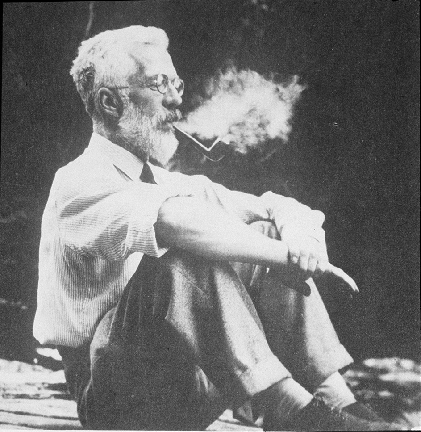
\includegraphics[width=0.4\textwidth]{figs/fisher1} \hspace{12pt} %\hfill
    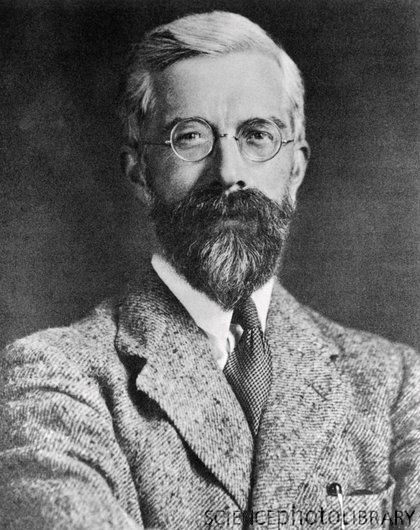
\includegraphics[width=0.4\textwidth]{figs/fisher2}
  \end{center}
  He was also a racist, sexist, and Nazi sympathizer.
\end{frame}




% \begin{frame}
%   \frametitle{Net reproductive rate ($R_0$)}
%   Net reproductive rate is the expected number of offspring that will
%   be produced by an individual during its lifetime.
% \[
%   R_0 = \sum_{i=1}^I f_i \prod_{j=1}^{i-1} s_j
% \]
% <<echo=false,results='hide'>>=
% f <- c(0, 0.5, 1.5, 1, 0.5, 0)
% s <- c(0.2, 0.3, 0.4, 0.4, 0.2, 0)
% R00 <- f[1]
% for(i in 2:length(f)) {
%     R00[i] <- f[i]*prod(s[1:(i-1)])
% }
% R0 <- sum(R00)
% @
% \end{frame}




% \begin{frame}
%   \frametitle{Generation time ($T$)}
%   Generation time is the time required for a population to increase
%   by a factor of $R_0$.
% \[
%   T = \frac{\log(R_0)}{\log(\lambda)}
% \]

% \end{frame}



\begin{frame}
  \frametitle{Other important quantities}
  {\bf Net reproductive rate \\}
  The expected number of individuals produced by an individual over its lifetime
  \[
    R_0 = \sum_{i=1}^I f_i \prod_{j=1}^{i-1} s_j
  \]
  \pause
  \vfill
  {\bf Generation time \\}
  The time required for a population to increase by a factor of $R_0$
  \[
    T = \frac{\log(R_0)}{\log(\lambda)}
  \]
\end{frame}





%% \begin{frame}
%%   \frametitle{Reproductive value}
%%   In a spreadsheet, there are two ways of calculating RV:
%%   inoculate
%%   transpose method
%% \end{frame}







%% \begin{frame}
%%   \frametitle{Generation time}
%%   The average age of a reproducing adult
%%   \[
%%     G = \sum_{y=0}^\infty l_y v_y
%%   \]
%% \end{frame}






%\begin{frame}
%  \frametitle{Concluding thoughts}
%  \Large
 % {\bf Future}
 % \begin{itemize}
 %   \item Sensitivity analysis: How does a change in $\theta$ affect $\lambda$?
 % \end{itemize}
 % \pause
%  {\bf Summary}
%  \begin{itemize}
%    \item In some cases, size may be better descriptor of variation in
%      demographics
%    \item We won't cover stage-based models
%    \item Individual variation within age classes is ignored.
%  \end{itemize}
%\end{frame}









\begin{frame}
  \frametitle{Other properties of the Leslie matrix\footnote{This is
      for graduate students only}}
  \Large
%  \begin{itemize}[<+->]
%  \item
  The dominant eigenvalue of ${\bf A}$ is the growth rate $\lambda$. \\
  \pause
  \vfill
  % \item
  The right eigenvector is the {\bf stable age distribution}. \\
  \pause
  \vfill
  % \item
  The left eigenvector is {\bf Fisher's reproductive value}. \\
%  \end{itemize}
\end{frame}





\section{Stage-structured models}






\begin{frame}
  \frametitle{Stage-structured population models}
  \begin{itemize}
    \item Age isn't always the best way to think about population structure
    \item<2-> For some populations, it is much more useful to think about size
      structure or even spatial structure.
    \item<3->  These ``stage-structured'' models differ from age-structured models
      in that individuals can remain in a stage class (with
      probability $1-p_i$) for multiple time periods.
  \end{itemize}
%  \vfill
  \tikzstyle{level 1} = [circle, draw, text width=0.5cm, minimum size=1.5cm,
  node distance=3cm, text centered, fill=blue!10]
  \begin{center}
   \uncover<4>{
   \begin{tikzpicture} \footnotesize %\small
      \node [level 1] (n1) [yshift=-5mm] {$n_{1,t}$};
      \node [level 1, right of=n1] (n2) [yshift=0mm] {$n_{2,t}$};
      \node [level 1, right of=n2] (n3) [yshift=0mm] {$n_{3,t}$};
      \draw[->,thick]  (n1) to node[above] {$s_1$} (n2);
      \draw[->,thick] (n2) to node[above] {$p_2s_2$} (n3);
      \draw[->,thick] (n2) to [bend right=40] node[above] {$f_2$} (n1);
      \draw[->,thick] (n3) to [bend right=60] node[above] {$f_3$} (n1);
      \draw[->,thick] (n2) to [loop below] node[below] {$(1-p_2)s_2$} (n2);
      \draw[->,thick] (n3) to [loop below] node[below] {$s_3$} (n3);
   \end{tikzpicture}
   }
  \end{center}
\end{frame}






%\begin{comment}
\begin{frame}
  \frametitle{Stage-structured population models}
  \large
  {In stage-structured models, individuals transition from one
    stage to the next with probability $p_i$. \par
    \vfill
    \pause
    We can add these
    transition probabilities to our projection matrix like this:}
  \pause
  \vfill
  \begin{center}
    \[
    {\bf A} =
    \begin{bmatrix}
      f_1 & f_2 & f_3 & f_4 \\
      s_1 & s_2(1-p_2) & 0 & 0 \\
      0 & s_2 p_2 & s_3(1-p_3) & 0 \\
      0 & 0 & s_3p_3 & s_4
    \end{bmatrix}
    \]
  \end{center}
%\pause
%\vfill
%This example allows for individual to remain in stages 2 and 3 for
%more than one time period.
\end{frame}
%\end{comment}







\begin{frame}
  \frametitle{Summary}
%  \begin{itemize}[<+->]
%  \item
  Vital rates ($s$ and $f$) are usually age-specific. \\
  \pause
  \vfill
  % \item
  Population growth will depend on age distribution. \\
  \pause
  \vfill
  % \item
  If vital rates are constant, population will reach stable
  age distribution with constant growth rate $\lambda$. \\
  \pause
  \vfill
  % \item
  Reproductive value indicates which age class contributes the
  most to population growth. \\
  \pause
  \vfill
  % \item
  Matrix models are a convenient method used to work with
  age-structured populations. \\
%  \end{itemize}
\end{frame}




\begin{comment}

\section{Sensitivity analysis}


\begin{frame}
  \frametitle{Sensitivity analysis}
  {\bf Questions}
  \begin{itemize}
    \item How will $\lambda$ change if we change $b$ or $d$?
  \end{itemize}

\end{frame}




%\begin{comment}
\section{Life Tables}


\begin{frame}
  \frametitle{Scenario}
  \large
  \begin{itemize}
    \item Age ($x$) begins at 0, ends at $k$
    \item The age class ($i$) begins at 1, and ends at $s=k-1$
  \end{itemize}
  \begin{center}
    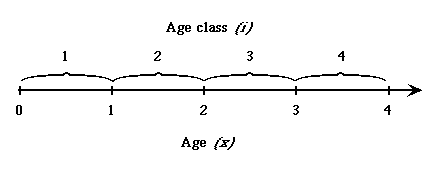
\includegraphics[width=0.6\textwidth]{figs/age-class-diagram}
  \end{center}
  \pause
  \begin{itemize}
    \item Individuals either advance to the next age class or die
    \item An age class is not necessarily a 1 year time period
    \item Each age class has its own vital rates
    \item We usually only care about females
  \end{itemize}
\end{frame}



\begin{frame}
  \frametitle{Life Tables}
  {\bf Assumptions}
  \begin{enumerate}[(1)]
    \item Birth-pulse model
      \begin{itemize}
        \item Individuals give birth on day they enter new age class
      \end{itemize}
    \item Postbreeding census
  \end{enumerate}
\end{frame}




\begin{frame}
  \frametitle{Life Tables}
  \begin{center}
    \begin{tabular}{cccccc}
      \hline
      Age ($x$) & Age class ($i$) & $b_x$ & $s_i$ & $l_x$         & $F_i$       \\
      \hline
      0         &                 & 0     &          & 1.0          & \\
      1         & 1               & 0.8   & 0.7      & $s_1$=0.7 & $b_1s_1$ \\
      2         & 2               &       & 0.7      & $s_1s_2$=   & \\
      \hline
    \end{tabular}
  \end{center}
  \begin{itemize}
    \item[] $b_x$ is the average number of offspring produced by an
      individual of age $x$
    \item[] $l_x$ is the probability of surviving from age 0 to age $x$
  \end{itemize}
\end{frame}






\note{Euler-Lotka equation: After stable age distribution is attained,
the population grows at a constant rate that is given by the solution
of the E-L equation. }







%% \begin{frame}
%%   \frametitle{Life tables in reverse}
%%   \note{On the assumption that the population is (1) at a stable age
%%     distribution and (2) stationary (i.e. $\lambda$=1, it may be
%%     possible to use the standing age distribution to calculate
%%     age-specific survival rates}
%%   \note{In general, it is not possible to use age frequency data alone
%%     to both estimate age-specific survival and to test the assumptions
%%     of age stability and stationarity.}

%% \end{frame}




\end{comment}





\end{document}
